\begin{figure*}[t]
\centering
\footnotesize
\resizebox{\textwidth}{!}{%
\begin{tikzpicture}[
  font=\footnotesize,
  lm/.style={draw=blue!55,fill=blue!6,rounded corners,align=left,
             text width=4.3cm,inner sep=3pt,minimum height=0.8cm},
  vlm/.style={draw=orange!75!black,fill=orange!8,rounded corners,align=left,
              text width=3.6cm,inner sep=3pt,minimum height=0.8cm},
  call/.style={-{Latex[length=2mm]},blue!55,thick},
  ret/.style={-{Latex[length=1.6mm]},orange!75!black,thin,dashed,opacity=0.7}
]
% lane headers
\node[font=\small\bfseries,blue!55!black] at (2.2,0.75) {Reasoner-LM \;(writes Python)};
\node[font=\small\bfseries,orange!70!black] at (7.4,0.75) {frozen VLM \;(\texttt{batch\_look})};

% reasoner-LM lane (left)
\node[lm]  (s1) at (2.2,0)    {\textbf{1. Survey} 10 candidate pages in one batched call};
\node[lm]  (s2) at (2.2,-1.2) {\textbf{2. Locate} via a table-of-contents pointer};
\node[lm]  (s3) at (2.2,-2.4) {\textbf{3. Read} page 76 (full page)};
\node[lm,draw=red!60,fill=red!5]  (s4) at (2.2,-3.75)
     {\textbf{4. Distrust \& verify:} crop to the chart and re-read};
\node[lm]  (s5) at (2.2,-5.1) {\textbf{5. Adjudicate:} re-read top \& bottom halves separately};
\node[lm,fill=blue!12]  (s6) at (2.2,-6.55)
     {\textbf{6. Compute in Python} (arithmetic the VLM cannot do):\\
      \texttt{2287.07 $-$ 238.19} $\Rightarrow$ \textbf{SUBMIT 2048.88} \checkmark};

% VLM lane (right of divider)
\node[vlm] (r1) at (7.4,0)     {per-page summaries};
\node[vlm] (r2) at (7.4,-1.2)  {``the table is on p.\,76''};
\node[vlm] (r3) at (7.4,-2.4)  {\$2{,}287.07 \,/\, \$238.19};
\node[vlm,draw=red!60] (r4) at (7.4,-3.75)
     {\$978.42 \,/\, \$190.57\\\textbf{(disagrees!)}};
\node[vlm] (r5) at (7.4,-5.1)  {\$2{,}287.07 \,/\, \$238.19 \;\checkmark};

% request (LM->VLM) and return (VLM->next LM) arrows
\foreach \i in {1,2,3,4,5} {
  \draw[call] (s\i.east) -- (r\i.west);
  \draw[ret]  (r\i.south west) .. controls +(-0.5,-0.35) and +(0.5,0.35) .. (s\the\numexpr\i+1\relax.east);
}
% lane divider
\draw[gray!35,dashed] (4.9,1.0) -- (4.9,-7.2);
\draw[gray!35,dashed] (9.5,1.0) -- (9.5,-7.2);

% ---- document thumbnails (the active-perception crop) ----
\node[inner sep=0,draw=gray!55] (pagefull) at (14.9,0.05)
     {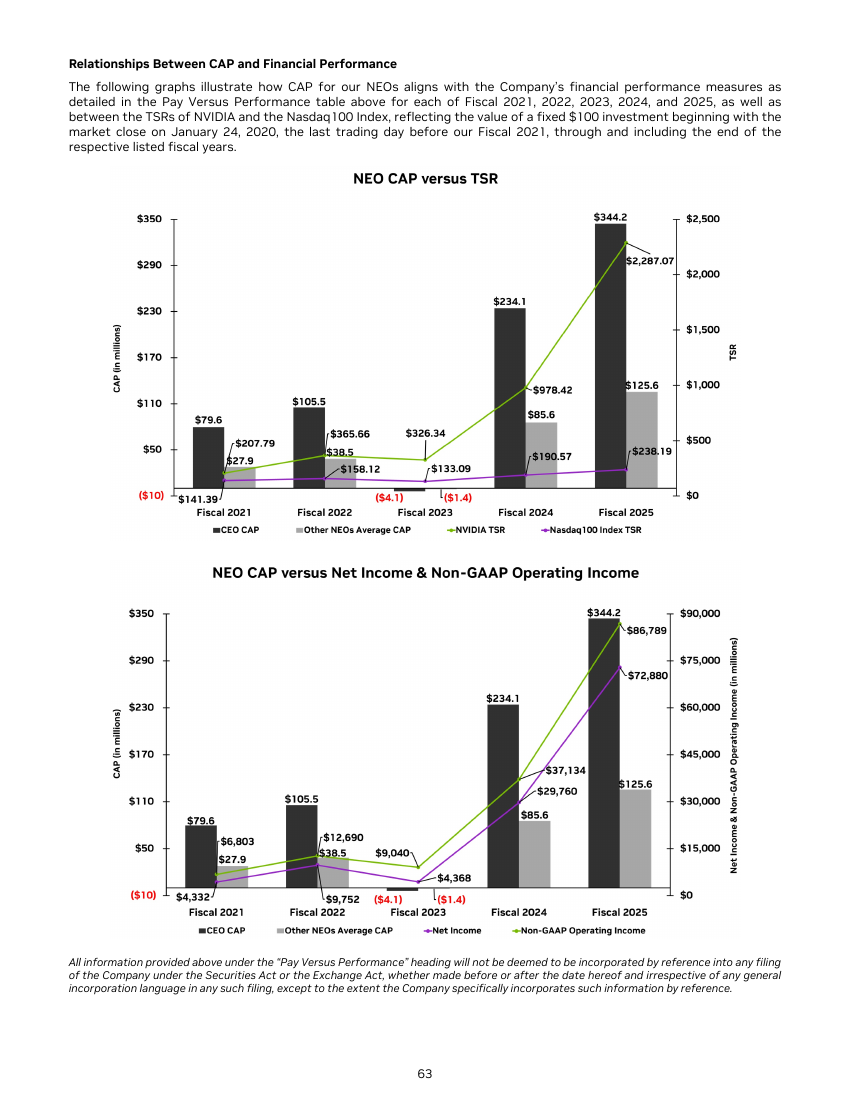
\includegraphics[height=2.4cm]{figs/br1_page76_full.png}};
\node[font=\scriptsize,gray!45!black,below=1pt of pagefull] {page 76 of 181};
\node[inner sep=0,draw=red!60,line width=0.7pt] (cropimg) at (12.9,-4.55)
     {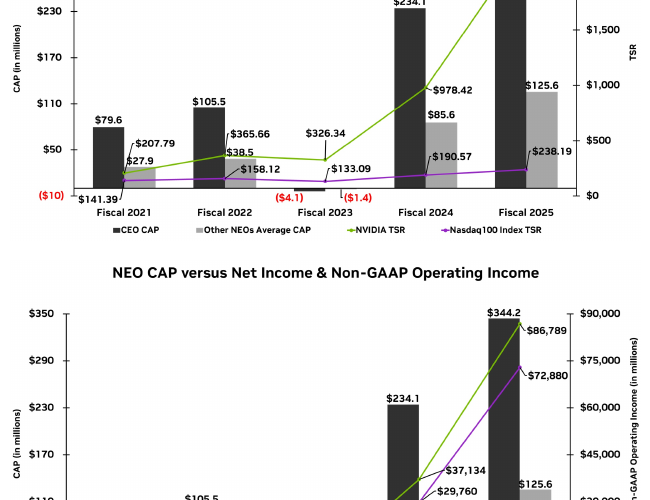
\includegraphics[width=4.7cm]{figs/br1_page76_crop.png}};
\node[font=\scriptsize,red!60!black,text width=5cm,align=center,above=1pt of cropimg]
     {the cropped chart band the agent re-read\\(the Fiscal 2025 bar is clipped off the top)};
\draw[call,-{Latex[length=2mm]}] (pagefull.south) -- node[right,font=\scriptsize,black]{crop \& zoom} (cropimg.north east);
\draw[red!60,dashed,-{Latex[length=2mm]}] (s4.north east) to[out=35,in=180] (cropimg.west);
\end{tikzpicture}%
}
\caption{Active-perception loop on a 181-page business report (NVIDIA annual review), RLM, 16 iterations, \textbf{correct} (gold and predicted 2048.88). Question: \emph{``In Fiscal 2025, by how many dollars does NVIDIA's TSR value exceed the Nasdaq-100 Index TSR value?''} The reasoner surveys the document, locates the table via a table-of-contents pointer, then \textbf{distrusts the full-page read and re-reads a tighter crop} (right) --- which disagrees, exposing a perception error --- adjudicates by reading the region in halves, and does the arithmetic in Python. Every component of the mechanism appears in one trace; the crop-verify catches a wrong number a single read would have submitted.}
\label{fig:trajectory}
\end{figure*}